% *******************************************************************************
% * Copyright (c) 2007 by Elexis
% * All rights reserved. This document and the accompanying materials
% * are made available under the terms of the Eclipse Public License v1.0
% * which accompanies this distribution, and is available at
% * http://www.eclipse.org/legal/epl-v10.html
% *
% *  $Id: abrechnung.tex 4911 2009-01-05 17:56:39Z rgw_ch $
%
%*******************************************************************************
% !Mode:: "TeX:UTF-8" (encoding info for WinEdt)

\section{'Views' en relation avec la facturation}
\subsection{Consultations selon date}
\begin{wrapfigure}{l}{7.3cm}
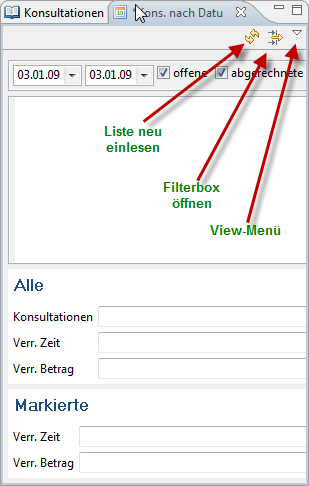
\includegraphics[width=7cm]{images/heute}
\caption{Konsultation nach Datum}
\label{fig:heute}
\end{wrapfigure}

Cette View (Fig. \ref{fig:heute}) sert à afficher les consultations d'une certaine période (normalement celles du jour actuel). Elle donne un aperçu de facturation et du temps calculé pour chaque consultation en particulier et aussi du total. En cliquant sur la 'check-box', vous pouvez laisser calculer des consultations ouvertes \footnote{il s'agit de celles qui n'ont pas encore été facturées} ou clôturées ou les deux. Vous pouvez indiquer dans les champs de date le début et la fin de la période en question. Après chaque modification vous devez utiliser le bouton 'actualiser liste' pour que la liste sera calculée à nouveau.

\medskip

Dans la section inférieure de la 'View' vous apercevez le nombre total des consultations au cours de la période choisie, ainsi que (défini par le système de codage de prestation) le temps et le montant comptabilisé. Dans le champ dessous vous voyez les mêmes indications pour la consultation actuellement marquée en bleu.

Vous pouvez donc utiliser cette 'View' aussi pour pouvoir passer revu le soir
toutes les consultations de la journée et pour introduire les prestations ou pour les corriger.


\medskip

En outre, cette 'View' permet des fonctions statistiques simples :
%\begin{itemize}
Si vous cliquez sur le bouton 'filtre', une boîte de filtre s'ouvre dans la partie supérieure de la 'View'. Depuis une fenêtre de facturation vous pouvez tirer les positions que vous voulez prendre en compte vers cette boite. Lors de la prochaine actualisation de la liste, la 'View' ne calculera que des consultations dans lesquelles apparaît au moins un des codes de positions souhaités. Les codes et les sommes totales seront alors énumérés séparément (lors de l'impression, voir ci-dessous).

\medskip

Dans 'view-menu' vous trouvez l'option 'imprimer liste'. En cliquant dessus, une fenêtre s'ouvre contenant un tableau qui énumère et fait imprimer les consultations indiquées.

\medskip

Pour des statistiques plus détaillées vous pouvez choisir aussi dans la'view-menu' l'option 'statistiques'. Ceci fourni un fichier en format CSV\footnote{Character Separated Values : un format standard pour des fichiers sous forme de tableau} qui peut être lu et statistiquement conditionné par des programmes comme OpenOfficde.org calc ou Microsoft\texttrademark Excel\texttrademark Ce fichier contient toutes les positions comptabilisées avec fréquence, coûts et chiffre d'affaire.


\subsection{Consultations à facturer}
\index{facturation} Cette View (cf Fig. \ref{fig:konsv})sert à choisir les consultations, dont une facture doit être établie.
Ceci concerne seulement les consultations du mandant actuel.

\begin{figure}[hb]
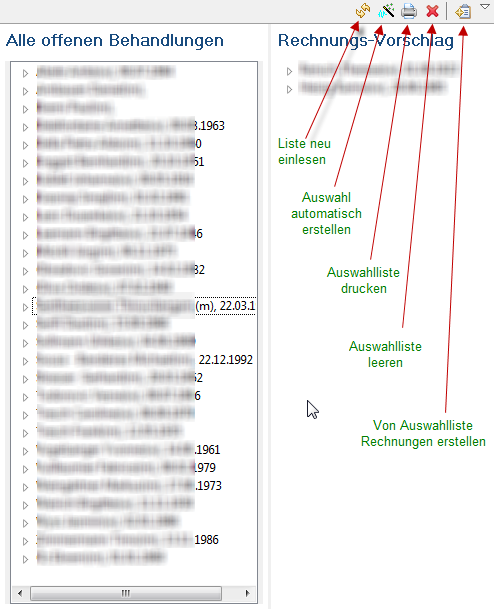
\includegraphics{images/konsv}
\caption{Konsultation zur Verrechnung auswählen}
\label {fig:konsv}
\end{figure}
Pour cela il y a des possibilités suivantes :
\begin{itemize}
  \item Choix automatique (Icône de baguette magique) : Les consultations à facturer sont choisies automatiquement d'après certaines règles et transférées dans la liste de choix. Cela sera expliqué ci-dessous plus précisément (facturation automatique).
  \item Tirer le nom du patient vers la liste de choix : Toutes les consultations concernant tous les cas (LAMAL , LAA etc) du patient choisi sont marquées pour être facturées.
  \item Tirer des cas (LAMA ; LAA etc) depuis la liste vers la liste de choix : Toutes les consultations des cas choisis sont marquées pour être facturées.
  \item Tirer des consultations depuis la liste vers la liste de choix : Seulement les consultations choisies sont marquées pour être facturées.
\end{itemize}
Avec toutes les méthodes mentionnées vous pouvez librement modifier votre choix postérieurement. Vous pouvez ajouter d'autres éléments, ou vous pouvez éliminer des éléments (après clic droit sur un élément dans la liste de choix), ou vous pouvez supprimer même le choix entier. A ce moment là il n'y a pas encore eu de modification des données .

Si vous avez fini de choisir vous pouvez cliquer sur  \glqq établir les factures\grqq pour que les factures pour tous les éléments présents dans le choix soient établies. Toutes les consultations qui font partie d'un cas sont toujours résumées. Plusieurs factures sont ainsi fournies si plusieurs cas d'un patient  se trouvent dans la liste de choix.

\subsubsection{Facturation automatique}
\index{Facturation automatique}\label{auto}
Par cette méthode la facturation des consultations suit des critères spécifiquement déterminés auparavant  (cf Fig. \ref{fig:rnautomatik}).
\begin{figure}
  % Requires \usepackage{graphicx}
  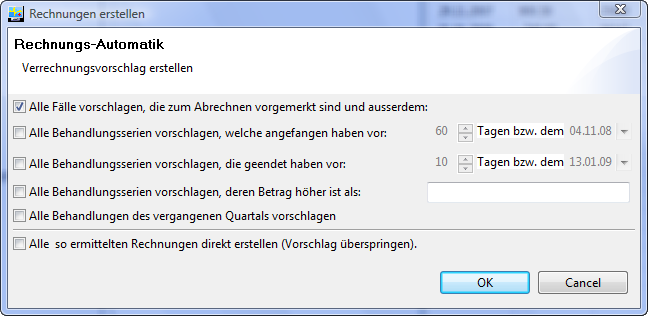
\includegraphics[width=1.0\textwidth]{images/rechnungsautomatik}\\
  \caption{Halbautomatischer Rechnungsvorschlag}\label{fig:rnautomatik}
\end{figure}

\begin{itemize}
\item Proposer tout les cas qui sont retenu pour la facturation : Si vous cliquez cette 'check-box' les consultations des cas seront choisis pour lesquels vous avez spécifié une date de facturation dans les détails du cas. (voir Fig. \ref{fig:falldetail}).
\item Proposer toutes les séries de traitement qui ont commencé avant le … : Choisit toutes les consultations non facturées d'un cas (LAMA, LAA etc) jusqu'aujourd'hui à condition qu'au moins une consultation avait eu lieu avant la date limite.
\item Proposer toutes les séries de traitement qui ont été terminées avant le … : Choisit toutes les consultations non facturées d'un cas (LAMA, LAA etc) à condition que la dernière consultation avait eu lieu avant la date limite.
\item Proposer toutes les séries de traitement dont la somme est plus grande que … : Choisit toutes les consultations non facturées d'un cas (LAMAL, LAA etc) à condition que la somme totale de la facture dépasse le montant choisi.
\item Proposer la facturation de tous les traitements du trimestre passé : Facturation du dernier \textit{trimestre} selon le calendrier avec les dates limites suivantes : 31.3 ; 30.6 ; 30.9 et 31.12.
\end{itemize}
S'applique à toutes les options : N'est exploitée seulement lorsque le crochet est mis dans la 'check-box'. Il ne suffit donc pas de seulement introduire une valeur. Les différentes options s'appliquent de façon additive : Finalement toute consultation est choisie pour la facturation à la quelle s'applique au moins un des critères actifs.

\medskip

\clearpage

\subsection{Factures}
\begin{figure}[ht]
  % Requires \usepackage{graphicx}
  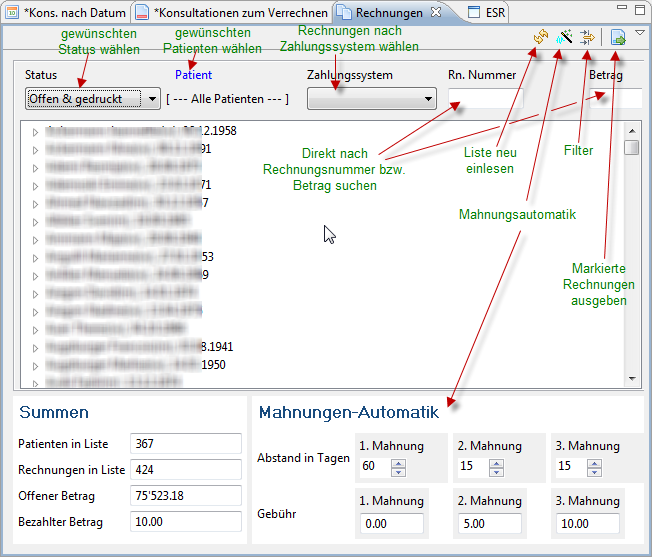
\includegraphics[width=1.0\textwidth]{images/rechnungsview}\\
  \caption{Rechnungen-View}\label{fig:rechnungen}
\end{figure}

Dans cette 'View' (Fig. \ref{fig:rechnungen})vous voyez les factures établies. Une facture a toujours un 'état' spécifique :
\begin{description}
    \item [Ouvert] immédiatement après la facturation. 
    \item [Ouvert et imprimé ] La facture avait été édité au moins une fois (soit par impression soit par une autre méthode d'exportation). A partir de ce moment le délai de payement commence à s'écouler. (Toutefois Elexis ne peut pas constater si par exemple une facture n'a pas été correctement imprimé ou si elle n'avait pas été envoyée. Pour cette raison se trouve ici une source d'erreurs potentielle.)
    \item[Rappel] Le rappel a été établi mais pas encore imprimé.
    \item[Rappel imprimé ] Le rappel a été imprimé.
    \item [2ième Rappel établi, 2ième Rappel imprimé, 3ième Rappel établi, 3ième Rappel imprimé ]: en analogie
    \item[Payement partiel ] Il y a au moins un payement mais qui ne couvre pas la totalité de la facture.
    \item[payée] La facture a été entièrement payée par un ou plusieurs paiements.
    \item [payé trop] ça peut aussi arriver pour une fois ;-)
    \item [Perte partielle ] Une partie de la facturation est définitivement mise dans les pertes (Contrairement à la situation du  \glqq payement partiel \grqq{} vous ne comptez plus avec un payement de plus)
    \item [Perte totale] La facture entière fait partie des pertes. 
    \item [En poursuite ] exactement ça
    \item [Annulé ] Une fois une facture établie, elle ne peut plus être supprimée. Cela doit être ainsi car sinon il serait possible que quelqu'un réclame une facture qui n'existe plus ou que quelqu'un veut des renseignements concernant une facture inexistante. Lorsqu'une facture est invalide pour une raison quelconque (erreurs, exonération du montant etc.) elle doit être annulée. L'annulation d'une facture a dans tous les aspects pratiques le même effet qu'une suppression à part du fait que le numéro de facture reste attribué et que la facture peut être examinée plus tard encore.
    \item [faux] Si un module de facturation constate qu'une facture contient des fautes (par ex. le module Trust-X pourrait réclamer qu'il y manquent certaines numéros EAN) la facture concernée reçoit le signe 'faux' et peut donc être corrigée.
    \item [à imprimer] Toutes les factures encore ouvertes mais pas encore imprimées de même que les rappels pas encore imprimés se trouvent dans cet état.
    \item [encours des crédits ] L'ensemble de tout des factures 'ouvertes et imprimées' , des 'rappels imprimés', des '2ième rappel imprimé' des '3ième rappel imprimé' des 'payements partiels' et des factures 'en poursuite'. Il s'agit donc de toutes les factures dont vous attendez encore un payement.
    \item [Stop des rappels ] exactement ça
\end{description}

La liste de facturation peut être sélectionné selon des différents critères. Pour mettre à jour la liste avec les données modifiées veuillez cliquer sur le bouton 'actualiser liste'. Pour afficher les factures d'un certain état veuillez choisir l'état en question sur le menu déroulant en haut à gauche sous 'état' (cf Fig. \ref{fig:rechnungen}). Pour afficher que la facture d'un patient spécifique cliquez sur \glqq patient\grqq{}. La boite de dialogue s'affiche pour vous laisser choisir les contacts. Introduisez la nom du patient et sélectionnez-le ensuite sur la liste. Cliquez sur o.k ou sur annuler pour retourner à l'affichage de la liste de tout les patients.

Pour ne choisir qu'un numéro de facture spécifique veuillez entrer le numéro dans le champ 'No de facture' et appuyez sur la touche 'Entrée' ou cliquez sur 'actualiser liste'.  Pour chercher une facture avec un montant spécifique (par ex. pour classer un payement de provenance non connue veuillez introduire le montant et poussez la touche d'entrée.

\medskip
Si vous cliquez sur le symbole 'filtre' vous recevez des options supplémentaires concernant l'affichage. 

\begin{wrapfigure}{l}{7cm}
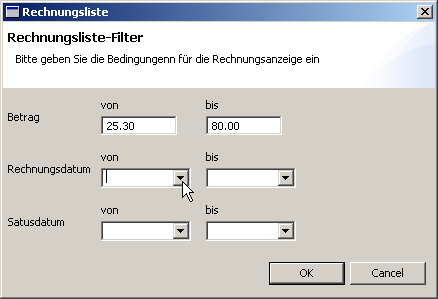
\includegraphics[width=7cm]{images/rechnungsfilter}
\end{wrapfigure}
Les champs 'Montant : de  - à' servent à filtrer une somme spécifique. Vous pouvez aussi remplir qu'un des deux champs de sorte que l'autre devienne un limitation ouverte.
 Les champs \glqq date de facturation de\grqq{} et \glqq date de facturation jusque\grqq{} servent à chercher des factures uniquement émises entre les deux dates mentionnées. Par contre les champs  \glqq dates d'état : de - à\grqq{} permettent à filtrer des factures dont la dernière modification d'état se trouve entre les deux dates introduites. Aussi ici vous pouvez remplir un seul champ et laisser l'autre ouvert. 
 Si vous sortez de ce dialogue en cliquant sur OK, la liste sera actualisés selon vos nouveaux critères.

\medskip

Tant que le bouton 'filtre' reste enclenché toutes les 'actualisations de liste' seront liés avec le Filtre ET. Si vous filtrez par exemple la date 'd'état' jusqu'au 30.10.2007 et vous cliquez après dans le menu déroulant sous 'état' sur '2ième rappel imprimé' et vous appuyez sur le bouton 'actualiser liste', vous trouverez toutes les factures qui avaient été mises avant le 30.10.2007 dans l'état '2ième rappel imprimé'. 

En bas de cette fenêtre vous voyez la quantité de factures qui remplissent ces conditions et les sommes les concernant.

\subsubsection{'View-menu' de la liste des factures}
Le 'View-menu' (triangle à droite en haut, cf Fig. \ref{fig:rechnungen}) a des options suivantes :
\begin{description}
\item [Affichage complet / Affichage réduit ] Montre toutes les donnés en détail ou les réduit aux titres.
\item [Imprimer liste ] Imprime une liste de tout les patients respectivement factures qui sont marquées dans l'affichage actuel. Pour cette action il faut qu'il y existe un modèle d'impression pour le système nommé 'liste' qui contient un champ (liste).
\end{description}
\subsubsection{Changer une facture}
Vous pouvez changer la facture si vous cliquez avec la touche droite de la souris sur une facture dans la liste :
\begin{description}
\item [Facturer] Facturer une facture séparée. (v. ci-dessous)
\item [Comptabiliser paiement ] Vous pouvez introduire ici les paiements manuellement . Par exemple des paiements comptants ou les paiements par acompte. (Normalement la comptabilisation par fichier ESR se fait automatiquement).
\item [Ajouter émolument ] Ajouter manuellement par ex. les frais de rappel.
\item [Changer l'état ] On peut changer l'état de la facture manuellement. Elexis reconnaît la majorité des changements de l'état d'une facture. Ainsi change l'état des factures payées automatiquement sur  \glqq payée\grqq{} lorsqu'un fichier ESR de la banque est comptabilisé. Certains changements de l'état ne peuvent se faire que manuellement. Par exemple : Elexis ne peut par distinguer automatiquement entre \glqq paiement partiel\grqq{} et \glqq perte partielle\grqq{} puisque ceci doit être lié à une décision du créancier. La même chose vaut pour les factures \glqq En poursuite\grqq{} et la \glqq perte totale\grqq{}.
    A part de ça il faudra toujours être prudent avec des changements manuelles de l'état d'une facture car il n'y se font pas de corrections de comptabilisation.
\item [Augmenter le niveau de rappel] Ceci augmente le niveau de rappel d'une étape jusqu'au maximum du 3ième rappel.
\item [Annuler] Ceci permet d'annuler une facture. Il y existe la possibilité de débloquer certains traitements (lorsque la facture était erronée et doit être refaite) ou de les laisser bloqués (si le traitement ne doit définitivement pas être facturé).
\end{description}

\subsubsection{Facturation}
Par le bouton  \glqq facturation\grqq{} toutes les factures sélectionnées seront facturées. (Pour sélectionner une facture cliquez avec la touche gauche de la souris sur la facture. Pour sélectionner plusieurs factures sur la liste cliquez sur ces factures en tenant enfoncée en même temps la touche CTRL (ou MAC). Pour marquer toute une rangée de factures cliquez d'abord sur la première facture et après, en tenant la touche SHIFT, sur la dernière facture de la rangée.) Elexis ne facturera donc \textit{pas} toute la liste mais seulement les factures sélectionnées de la liste !


Les cibles possibles de la facturation dépend des différents 'Plugins de facturation' installés.
La cible peut par exemple être une imprimante qui imprime des factures selon TARMED, mais elle peut aussi être un fichier XML ou directement un centre de confiance. Des informations plus précises vous pouvez trouver dans les chapitres respectives  (Tarmed: page \pageref{arzttarife}).
\bigskip
En cliquant sur le symbole de la baguette magique vous mettez en route l'automatisme de l'établissement des rappels. Celle-ci choisit les factures à rappeler selon les critères fixés dans le champ en bas à droite, augmente le niveau de rappel, ajoute des émoluments comme prédéterminé et réunit ces factures en groupes  \glqq à imprimer\grqq{}.

\subsection{Compte du patient}
\index{Compte}Cette 'View' permet de voir tous les mouvements de compte du patient. Les factures se comptabilisent par des chiffres négatifs, les paiements ou annulations par des chiffres positifs de sorte que vous puissiez apercevoir facilement et à travers plusieurs facturations et paiements où vous en êtes avec ce client du point de vu financier.

\subsection{Liste des comptes des patients}
Cette liste permet de voir tous les mouvements de compte en même temps.

\subsection{Prestations}
Cette 'View' fonctionne de façon semblable comme la 'View-Diagnostics'  (page \ref{view:diagnosen} à la page \pageref{view:diagnosen}): Dépendant des Plugins pour le codage des prestations installés on trouve pour chaque système de codage un onglet . Pour des précisions veuillez consulter \ref{concept:leistung} à la page \pageref{concept:leistung}.



